\newpage
% ==========================================
%              CHAPTER FIVE
% ==========================================
\thispagestyle{plain}

\begin{center}
    \vspace*{0.5cm}
    {\large \textit{Chapter Five}} \\[0.4cm]
    {\Large \textbf{5 \quad SYSTEM IMPLEMENTATION}}
\end{center}
\addcontentsline{toc}{chapter}{\textbf{5 \quad SYSTEM IMPLEMENTATION}}
\vspace{0.45in}

\normalsize
\startchapterfloats{5}

% Framed screenshot placeholder: swap for \includegraphics when the
% screenshot is ready. #1 = box height, #2 = description shown in box.
\newcommand{\imgplaceholder}[2]{%
  \fbox{\parbox[c][#1][c]{0.92\textwidth}{\centering
    \textbf{[INSERT IMAGE]}\\[4pt] \small #2}}}

\noindent Chapters~3--4 detailed the design, feature engineering, and architecture of the four standalone recognition models. This chapter documents how those models are wrapped into \textbf{Eshara}, a deployable web application, and describes the surrounding product engineering: architecture, frontend, backend, database, real-time communication, security, and testing. The web application is the primary interface through which a user reaches the underlying deep-learning models for American Sign Language (ASL) and Arabic Sign Language (ArSL); it processes standard webcam input directly in the browser, requiring no dedicated hardware or native application install~\cite{fastapi,react,vite2024}. Graduation deployment scope is \textbf{web-only} --- no native mobile application, sensor gloves, or depth cameras~\cite{typescript2024}. The chapter is presented in two parts: \textbf{Part~A} (Sections~5.1--5.13) documents the core application --- system architecture, frontend, backend, database, translation workflow, security, deployment, and measured performance; \textbf{Part~B} (Section~5.14) documents the \textbf{Education Module} --- the bilingual Sign Viewer, Sentence Builder, and Practice tools built on motion-capture skeleton playback --- at the same technical depth.\par\vspace{0.3cm}

\begin{center}{\large \textbf{PART A --- CORE APPLICATION}}\end{center}
\vspace{0.1cm}

\noindent\textbf{5.1\quad SYSTEM ARCHITECTURE}\par
\addcontentsline{toc}{section}{\numberline{5.1}SYSTEM ARCHITECTURE}
\vspace{0.2cm}

\noindent Eshara adopts a \textbf{decoupled, three-tier architecture} so that computationally heavy machine-learning inference does not interfere with the responsiveness of the user interface or the core backend services:
\begin{enumerate}
\item \textbf{Client Tier (Frontend)} --- a responsive interface built with React and bundled with Vite~\cite{react,vite2024}, responsible for capturing the user's webcam stream and drawing educational stickman animations. It communicates with the backend over RESTful APIs for translation requests and over Socket.IO for real-time chat~\cite{socketio2024}.
\item \textbf{Application Tier (Backend API)} --- a Node.js and Express application~\cite{nodejs2024,expressjs2024} that acts as the secure gateway: it manages user authentication (JSON Web Tokens), session state, and database access through the Prisma ORM~\cite{prisma2024,rfc7519}, and proxies \texttt{/predict} requests from the client to the internal model service, hiding the ML environment from the public-facing client.
\item \textbf{Inference Tier (Model Services)} --- a dedicated FastAPI (Python) service~\cite{fastapi,uvicorn2024} that hosts the standalone translation models behind a single \texttt{/predict} endpoint, decodes base64-encoded frames or MediaPipe landmark vectors, and returns predicted text with a confidence score. It also manages generation and serving of \texttt{.pose} files consumed by the frontend's full-body word-sign visualisation.
\end{enumerate}
\vspace{0.2cm}

\noindent \textbf{Data-flow summary.} The user's webcam feed is sampled on the client as a base64-encoded JPEG and sent via an HTTP \texttt{POST} to the Application Tier. The Node.js server authenticates the request and forwards the payload internally to the Inference Tier. FastAPI runs the model appropriate to the requested language/mode combination (MLP for letters, BiLSTM or I3D for words) and the resulting prediction is propagated back through Node.js to the React interface in real time.\par\vspace{0.2cm}

\begin{figure}[H]
\centering
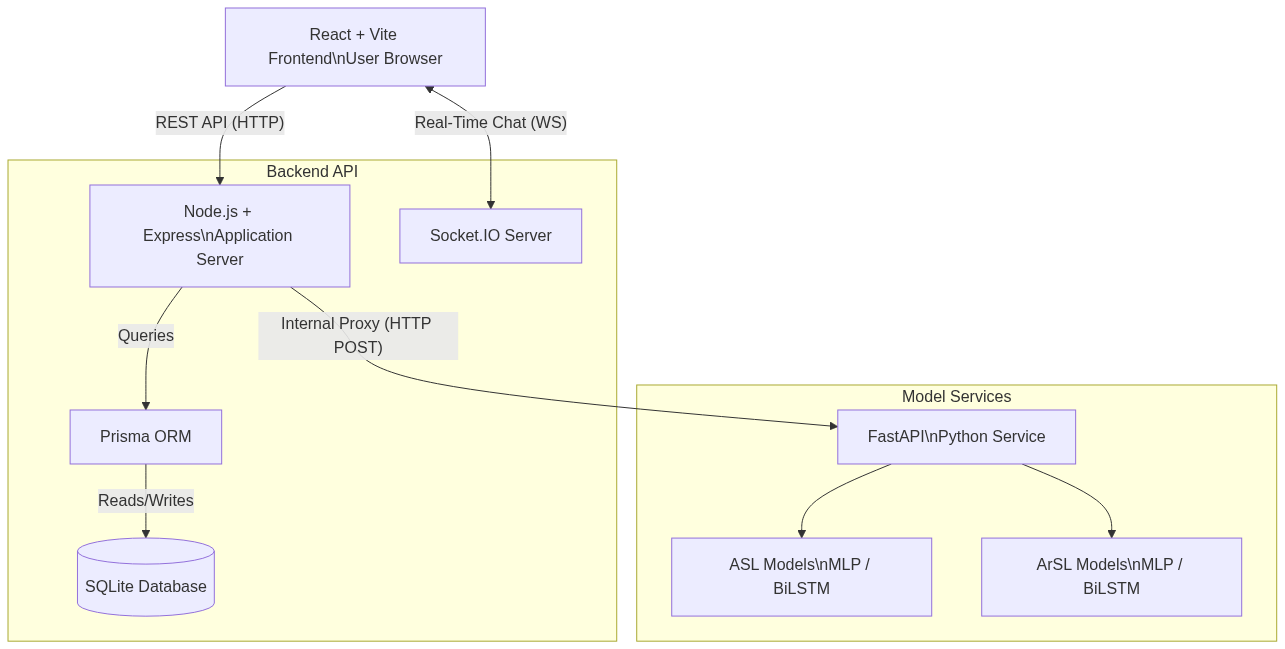
\includegraphics[width=1.00\textwidth]{images/fig_7-1_system_architecture.png}
\caption{Eshara three-tier system architecture: React/Vite client, Node.js + Express application server (Prisma ORM over SQLite, Socket.IO server), and the FastAPI model-services tier hosting the ASL/ArSL letter and word models.}
\label{fig:ch7-architecture}
\end{figure}
\vspace{0.2cm}

\noindent Within this deployment topology, the client only ever talks to the Node.js application server; the FastAPI inference tier is not exposed to the public internet, which both simplifies the client's networking surface and centralises CORS and validation policy in one place (Section~5.10).\par\vspace{0.2cm}

\begin{figure}[H]
\centering
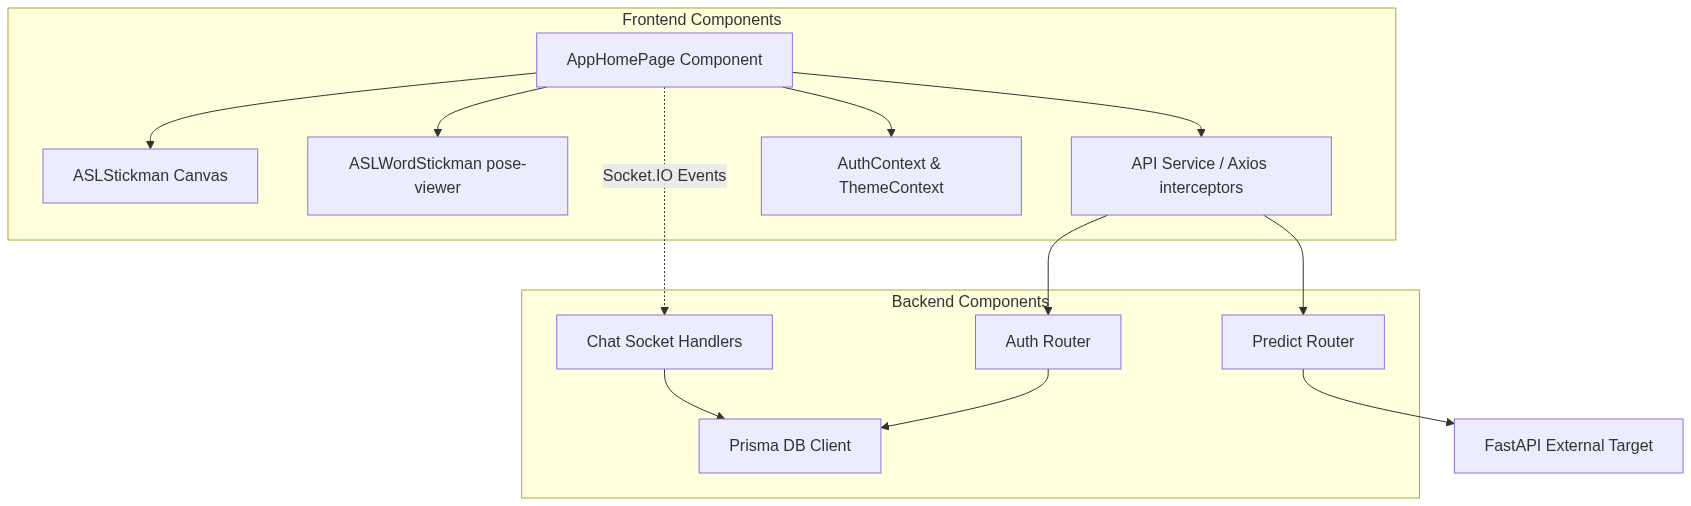
\includegraphics[width=1.00\textwidth]{images/fig_7-2_component_diagram.png}
\caption{Component diagram: frontend modules (\texttt{AppHomePage}, stickman/\texttt{pose-viewer} visualisers, \texttt{AuthContext}/\texttt{ThemeContext}, Axios service layer) and their dependencies on backend components (chat socket handlers, auth router, predict router, Prisma client, and the external FastAPI target).}
\label{fig:ch7-component}
\end{figure}
\vspace{0.3cm}

\noindent\textbf{5.2\quad FRONTEND DESIGN}\par
\addcontentsline{toc}{section}{\numberline{5.2}FRONTEND DESIGN}
\vspace{0.2cm}

\noindent The client is a Single Page Application (SPA) built with React and bundled by Vite for fast hot-module replacement and optimised delivery. The design methodology centres on reusable components, centralised state management, and a lightweight vanilla styling system rather than a heavy CSS framework.\par\vspace{0.2cm}

\noindent\textbf{5.2.1\quad State and component architecture:}\par
\addcontentsline{toc}{subsection}{\numberline{5.2.1}State and component architecture:}
\vspace{0.2cm}

\noindent Global application state --- user authentication sessions and UI theme preference --- is managed through React Context (\texttt{AuthContext} and \texttt{ThemeContext}), avoiding prop-drilling and keeping the UI synchronised across views. Main pages (\texttt{LandingPage}, \texttt{AppHomePage}) handle routing and high-level logic, while discrete components such as \texttt{ASLWordStickman} (the Sign Viewer), \texttt{SentenceBuilder}, and \texttt{PracticePanel} encapsulate the more complex playback and capture logic.\par\vspace{0.2cm}

\noindent\textbf{5.2.2\quad Styling and theming:}\par
\addcontentsline{toc}{subsection}{\numberline{5.2.2}Styling and theming:}
\vspace{0.2cm}

\noindent The application uses vanilla CSS (\texttt{index.css}) with CSS custom properties to define a shared design system for colours, gradients, and typography (Outfit font family), avoiding the overhead of a component-styling framework. A root-level \texttt{data-theme} attribute is toggled dynamically to switch between a dark mode and a high-contrast light mode, supporting usability under varying lighting conditions.\par\vspace{0.2cm}

\clearpage
\noindent\textbf{5.2.3\quad Education module interface:}\par
\addcontentsline{toc}{subsection}{\numberline{5.2.3}Education module interface:}
\vspace{0.2cm}

\noindent A core feature of the frontend is the \textbf{Educational} interface, which teaches sign language through two complementary mechanisms:
\begin{itemize}
\item \textbf{Sign playback (\texttt{<pose-viewer>})} --- all word signs, fingerspelling, and free-text sentences render as motion-capture skeleton animations of real signers, assembled server-side by the model-services tier and played by the \texttt{<pose-viewer>} web component~\cite{signmt2023,poseformat}.
\item \textbf{Practice capture (\texttt{useCamera})} --- a webcam practice panel reuses the same capture-and-\texttt{/predict} pipeline as the Chatting tab through a shared \texttt{useCamera} hook, with its own camera instance so the two tabs never interfere.
\end{itemize}
The module's full architecture --- content pipeline, server-side animation stitching, bilingual behaviour, and verification methodology --- is documented in Section~5.14 (Part~B).
\vspace{0.2cm}

\noindent\textbf{5.2.4\quad Webcam capture and layout:}\par
\addcontentsline{toc}{subsection}{\numberline{5.2.4}Webcam capture and layout:}
\vspace{0.2cm}

\noindent A responsive grid layout houses the live translation interface, which interacts with the browser's \texttt{navigator.mediaDevices} API~\cite{w3c2023html} to let the user select a specific camera input. The video stream is drawn to a horizontally inverted \texttt{<video>} element, acting as a mirror so the user receives intuitive visual feedback before a frame is sampled and sent to the backend.\par\vspace{0.3cm}

\noindent\textbf{5.3\quad BACKEND INTEGRATION AND AUTHENTICATION}\par
\addcontentsline{toc}{section}{\numberline{5.3}BACKEND INTEGRATION AND AUTHENTICATION}
\vspace{0.2cm}

\noindent\textbf{5.3.1\quad Core application server:}\par
\addcontentsline{toc}{subsection}{\numberline{5.3.1}Core application server:}
\vspace{0.2cm}

\noindent The backend is built with Node.js and Express~\cite{nodejs2024,expressjs2024} and acts as the central middleware and routing layer. Modular Express routers expose RESTful endpoints (\texttt{/auth}, \texttt{/users}, \texttt{/predict}, \texttt{/health}), keeping route concerns cleanly separated. To encapsulate the ML environment, the \texttt{predict} controller receives prediction requests (base64 image payloads, requested language and mode) and proxies them asynchronously to the internal FastAPI service, which hides the ML application's network ports from the public client and centralises CORS and validation policy in the Node.js layer.\par\vspace{0.2cm}

\noindent\textbf{5.3.2\quad Authentication infrastructure:}\par
\addcontentsline{toc}{subsection}{\numberline{5.3.2}Authentication infrastructure:}
\vspace{0.2cm}

\noindent Authentication is stateless and based on JSON Web Tokens~\cite{rfc7519}. On registration and login, passwords are hashed with \texttt{bcryptjs} using a high salt-round count before database insertion~\cite{bcrypt2024}; on successful authentication the server issues a cryptographically signed JWT payload carrying the user's ID and email. The React client stores this token and injects it as an \texttt{Authorization: Bearer} header on every outbound request via a custom Axios interceptor~\cite{axios2024}; a \texttt{401 Unauthorized} response causes the interceptor to purge the local token and route the user back to the login gateway.\par\vspace{0.2cm}
\clearpage
\noindent\textbf{5.3.3\quad Real-time communication (Socket.IO):}\par
\addcontentsline{toc}{subsection}{\numberline{5.3.3}Real-time communication (Socket.IO):}
\vspace{0.2cm}

\noindent Live chat and messaging use a Socket.IO server~\cite{socketio2024} layered over the core HTTP instance. The connection handshake is intercepted to validate the JWT before a socket is admitted, immediately dropping unauthorised connections and preventing access to private room broadcasts. Custom event emitters (\texttt{chat:join}, \texttt{chat:send}, \texttt{chat:receive}) deliver messages and UI updates instantaneously, avoiding the latency and overhead of HTTP polling.\par\vspace{0.3cm}

\noindent\textbf{5.4\quad DATABASE DESIGN}\par
\addcontentsline{toc}{section}{\numberline{5.4}DATABASE DESIGN}
\vspace{0.2cm}

\noindent\textbf{5.4.1\quad Prisma ORM and SQLite:}\par
\addcontentsline{toc}{subsection}{\numberline{5.4.1}Prisma ORM and SQLite:}
\vspace{0.2cm}

\noindent Persistence uses the Prisma ORM~\cite{prisma2024} paired with an SQLite database~\cite{sqlite2024}, giving an auto-generated, type-safe database client and rapid schema iteration without the overhead of running a standalone database server. The schema (\texttt{schema.prisma}) defines four models --- \texttt{User}, \texttt{Room}, \texttt{RoomMember}, and \texttt{Message} --- with strict foreign-key constraints and cascading deletes, so that deleting a room automatically removes its associated memberships and messages rather than leaving orphaned rows.\par\vspace{0.2cm}

\begin{figure}[H]
\centering
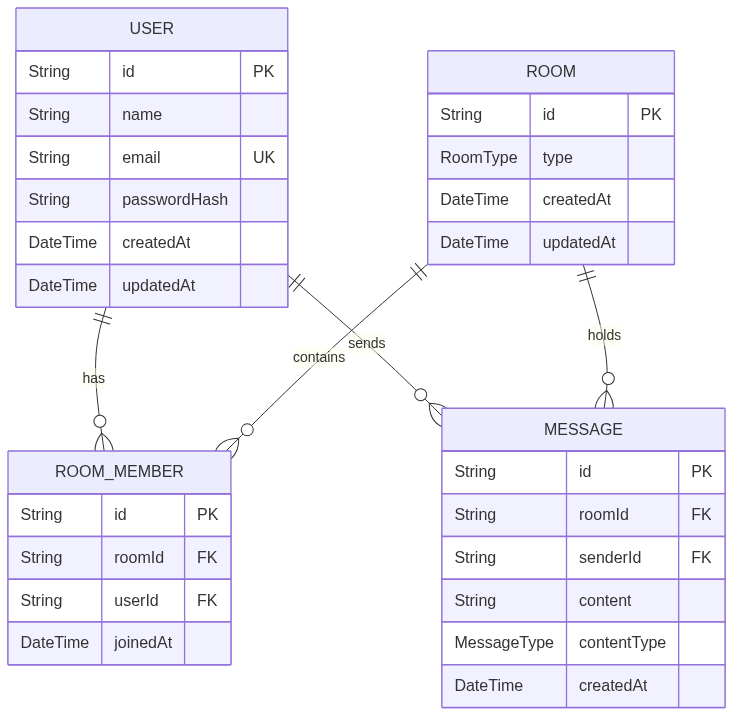
\includegraphics[width=0.95\textwidth]{images/fig_7-4_erd.png}
\caption{Entity--Relationship Diagram (ERD): \texttt{User}, \texttt{Room}, \texttt{ROOM\_MEMBER}, and \texttt{MESSAGE} tables with primary/foreign keys and cascading relationships, as defined in \texttt{schema.prisma}.}
\label{fig:ch7-erd}
\end{figure}
\vspace{0.2cm}

\noindent\textbf{5.4.2\quad Chat and message models:}\par
\addcontentsline{toc}{subsection}{\numberline{5.4.2}Chat and message models:}
\vspace{0.2cm}

\noindent A \texttt{RoomType} enumeration (\texttt{DIRECT} vs.\ \texttt{GROUP}) supports both one-to-one and multi-user chat configurations. The \texttt{Message} model additionally carries a \texttt{MessageType} enumeration (\texttt{TEXT}, \texttt{PREDICTION}, \texttt{SYSTEM}), letting the frontend distinguish manually typed text from strings produced by the AI translation engine and style them differently in the chat UI.\par\vspace{0.2cm}

\begin{figure}[H]
\centering
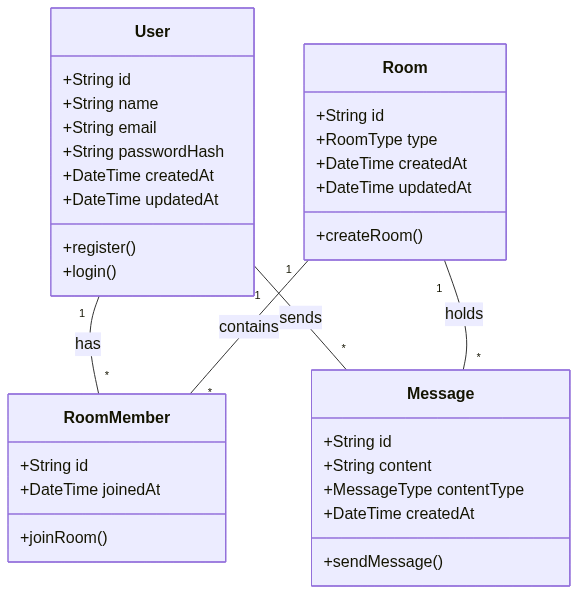
\includegraphics[width=0.95\textwidth]{images/fig_7-5_class_diagram.png}
\caption{Class diagram of the application-server domain objects (\texttt{User}, \texttt{Room}, \texttt{RoomMember}, \texttt{Message}) and their principal operations (\texttt{register()}, \texttt{login()}, \texttt{createRoom()}, \texttt{joinRoom()}, \texttt{sendMessage()}).}
\label{fig:ch7-class}
\end{figure}
\vspace{0.3cm}

\clearpage

\noindent\textbf{5.5\quad TRANSLATION WORKFLOW AND AI MODEL COMMUNICATION}\par
\addcontentsline{toc}{section}{\numberline{5.5}TRANSLATION WORKFLOW AND AI MODEL COMMUNICATION}
\vspace{0.2cm}

\noindent\textbf{5.5.1\quad Image capture and encoding:}\par
\addcontentsline{toc}{subsection}{\numberline{5.5.1}Image capture and encoding:}
\vspace{0.2cm}

\noindent The inference workflow begins on the React frontend: when the user requests a translation, a frame is synchronously captured from the active \texttt{<video>} element, drawn onto a hidden \texttt{<canvas>}, and encoded as a JPEG base64 string. This compression reduces payload size while preserving enough pixel detail for accurate landmark extraction downstream.\par\vspace{0.2cm}

\noindent\textbf{5.5.2\quad Cross-service communication:}\par
\addcontentsline{toc}{subsection}{\numberline{5.5.2}Cross-service communication:}
\vspace{0.2cm}

\noindent The encoded base64 string, together with the user's selected configuration metadata (language: ASL/ArSL; mode: letters/words), is dispatched to the Node.js \texttt{/predict} endpoint. The server authenticates the JWT and, on success, proxies the payload directly to the FastAPI model service over an internal HTTP request, acting as a secure intermediary that keeps the ML service address out of client-visible network traffic.\par\vspace{0.2cm}
\begin{figure}[H]
\centering
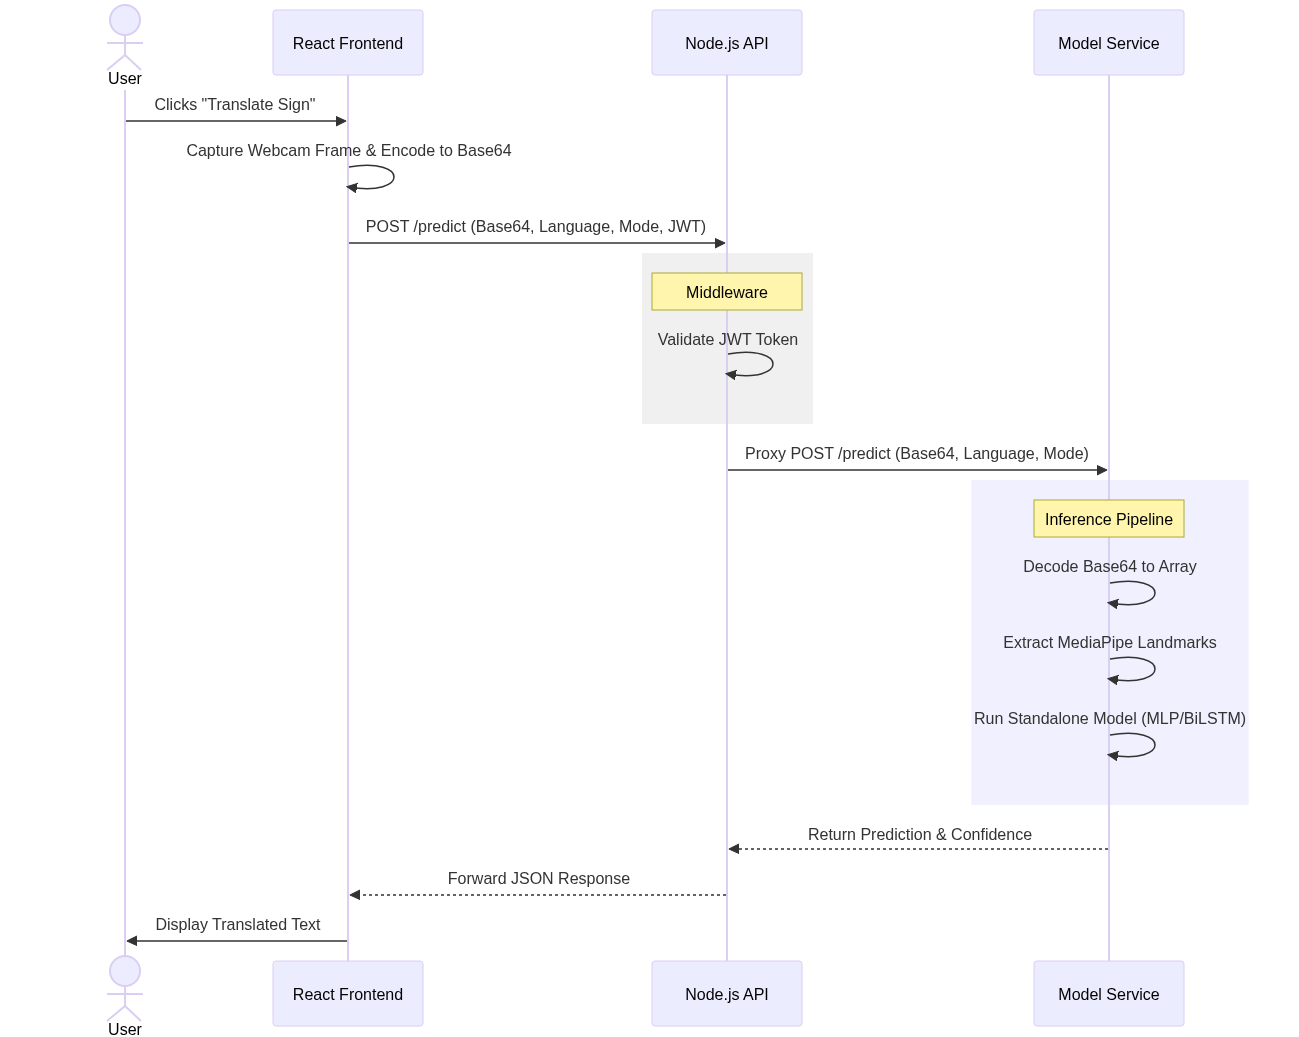
\includegraphics[width=0.925\textwidth]{images/fig_7-3_sequence_diagram.png}
\caption{Sequence diagram of the end-to-end translation request: React client $\rightarrow$ Node.js API (JWT validation) $\rightarrow$ FastAPI model service (MediaPipe landmark extraction, model inference) $\rightarrow$ JSON response relayed back to the client.}
\label{fig:ch7-sequence}
\end{figure}
\vspace{0.2cm}

\noindent\textbf{5.5.3\quad Model inference pipeline:}\par
\addcontentsline{toc}{subsection}{\numberline{5.5.3}Model inference pipeline:}
\vspace{0.2cm}

\noindent Upon receiving the payload, the FastAPI service interprets the request body's \texttt{language} (\texttt{en} | \texttt{ar}) and \texttt{mode} (\texttt{letters} | \texttt{words}) fields to instantiate the appropriate inference engine. In letter mode, incoming base64 imagery is routed to either \texttt{asl\_\allowbreak mlp\_\allowbreak inference.py} (English) or \texttt{arsl\_\allowbreak mlp\_\allowbreak inference.py} (Arabic). These modules perform real-time MediaPipe hand-landmark extraction and execute the corresponding MLP classifier (defined in Chapter~3 using 63-D/78-D features) to predict the highest-confidence character. Finally, the service packages the prediction into a JSON response, which is relayed through the Node.js API to the React client for injection into the user's input buffer or live-chat stream.\par\vspace{0.3cm}

\noindent\textbf{Word-mode integration status.} At the time of writing, the \texttt{english + words} combination is routed to the WLASL Inception I3D engine described in Section~5.6; the \texttt{arabic + words} combination is not yet wired to the deployed ArSL BiLSTM (Chapter~4, Model~4) inside this web application and currently falls back to a mock response, even though the underlying 225-D BiLSTM checkpoint is fully trained and evaluated offline at 99.62\,\% Top-1 (Chapters~6--7). Wiring the ArSL word model into \texttt{model-services} following the same \texttt{predict\_word(session\_id, image\_base64)} contract used for WLASL (Section~5.6) is listed as near-term integration work in Chapter~9.\par\vspace{0.3cm}

\noindent\textbf{5.6\quad ASL WORD MODEL INTEGRATION (WLASL / INCEPTION I3D)}\par
\addcontentsline{toc}{section}{\numberline{5.6}ASL WORD MODEL INTEGRATION (WLASL / INCEPTION I3D)}
\vspace{0.2cm}

\noindent The English word-recognition path required a different integration pattern from the landmark-based letter and ArSL-word models, because the ASL word model (Chapter~4, Model~3) is a PyTorch Inception I3D network consuming RGB clips rather than MediaPipe landmark vectors~\cite{carreira2017i3d,pytorch2024,li2020wlasl}. This work was carried out on a dedicated \texttt{add-wlasl-model} integration branch of the web application so that the stable \texttt{main} branch remained untouched while the RGB pipeline was wired in.\par\vspace{0.2cm}

\noindent\textbf{Migrated artifacts.} The FastAPI \texttt{model-services} package was extended with the I3D network definition, the pretrained 100-word checkpoint (\texttt{asl100.pt} / \texttt{asl\_word\_i3d.pt}), the WLASL gloss-to-index list, and \texttt{torch}/\texttt{torchvision} runtime dependencies (Chapter~4, Table~\ref{tab:ch4-artifacts}).\par\vspace{0.2cm}

\noindent\textbf{Stateful inference.} A dedicated \texttt{wlasl\_inference.py} module keeps one state dictionary per \texttt{session\_id} (a 32-frame deque, a 10-prediction voting window, last-commit timestamp, and last-committed word), so that multiple concurrent users are not confused with one another's clips. Each incoming frame is decoded, colour-converted, resized so its short side is 256\,px, centre-cropped to 224$\times$224, and mapped to $[-1,1]$ (the same preprocessing as Chapter~4, Figure~\ref{fig:ch4-asl-preprocess}) before being appended to that session's deque. 


\clearpage
\noindent\ Once 32 frames are buffered, the I3D network runs and its softmax output is pushed into a \textbf{10-prediction voting window}; a class is only \textbf{committed} once it is the majority vote in that window ($\geq$6/10), its confidence is $\geq$50\,\%, and at least 1.2\,s have passed since the last commit (mirroring the letter stabilisation decoder pattern from Chapter~3, Section~3.6) --- otherwise the endpoint reports a \texttt{buffering} status with the current best guess. On the Node.js side, the \texttt{predict} controller attaches the authenticated user's ID (\texttt{req.user.id}, or \texttt{"anonymous"} if the request is unauthenticated) as the \texttt{sessionId} forwarded to FastAPI, giving each logged-in user an isolated video buffer without the frontend having to manage session identifiers itself.\par\vspace{0.2cm}

\noindent\textbf{Routing.} The FastAPI \texttt{/predict} route was extended so that a request with \texttt{language="en"} and \texttt{mode="words"} is routed to the \texttt{wlasl\_inference} engine instead of a placeholder response, mirroring the same language/mode dispatch pattern already used for the letter MLPs (Section~5.5.3). This keeps a single request contract (\texttt{language}, \texttt{mode}, \texttt{imageBase64}) across all four models even though the ASL word path is architecturally the odd one out --- RGB frames rather than landmarks, and per-session server-side buffering rather than a single-frame forward pass.\par\vspace{0.3cm}

\noindent\textbf{5.7\quad NAVIGATION FLOW AND MAIN PAGES}\par
\addcontentsline{toc}{section}{\numberline{5.7}NAVIGATION FLOW AND MAIN PAGES}
\vspace{0.2cm}

\noindent The frontend uses \texttt{react-router-dom}~\cite{reactrouter2024} to govern navigation, with a flow that is linear and strictly gated by authentication status. Unauthenticated users land on the \textbf{Landing Page}, which presents an overview of the system and forms to register or log in. A custom \texttt{ProtectedRoute} higher-order component wraps the core application paths; if a user without a valid JWT attempts to reach the main dashboard, the router intercepts the navigation and redirects back to the Landing Page. Once authenticated, users are routed to the \textbf{App Home Page}, the central hub of the application, whose layout is split into two tabs: \textit{Chatting} (live translation and real-time messaging) and \textit{Educational} (sign-language visualisation and practice).\par\vspace{0.2cm}

\begin{figure}[H]
\centering
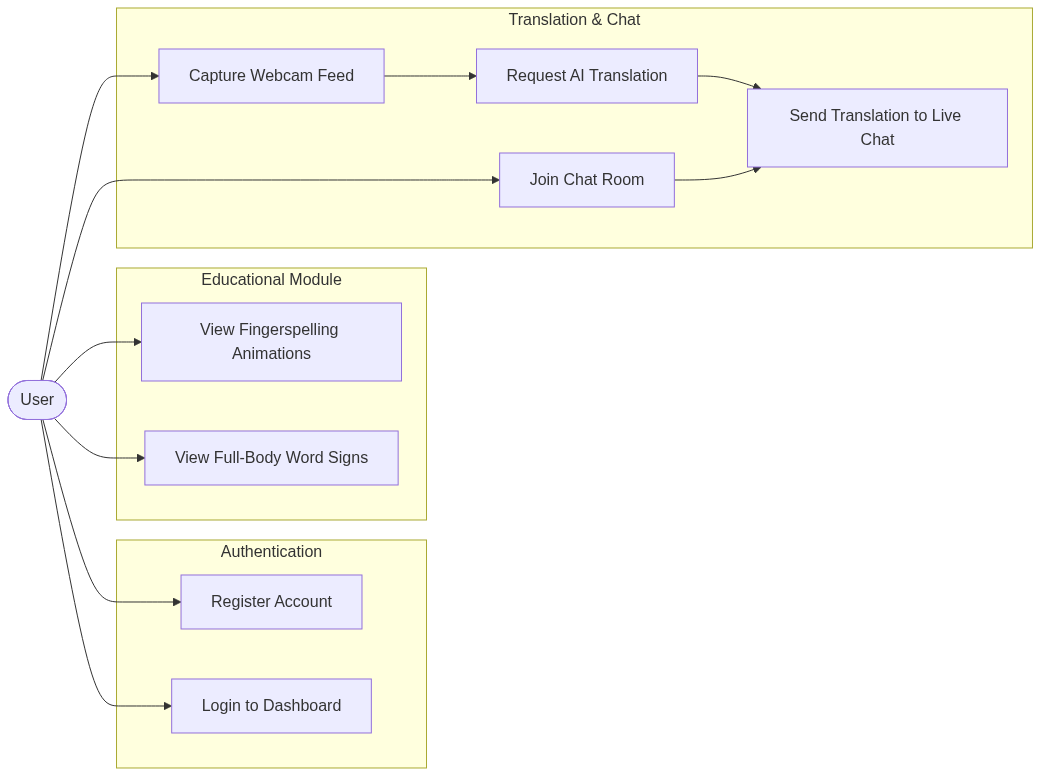
\includegraphics[width=1.00\textwidth]{images/fig_7-6_use_case.png}
\caption{Use case diagram: authentication (register/login), the Educational module (browse and watch word signs, fingerspell typed text, sign a typed sentence, practise signs with webcam feedback), and Translation \& Chat (capture webcam feed, request AI translation, join chat room, send translation to live chat).}
\label{fig:ch7-usecase}
\end{figure}
\vspace{0.3cm}

\noindent\textbf{Deployed web interface.} Figures~\ref{fig:ch7-login} and~\ref{fig:ch7-apphome} show the live Eshara web application. The \textbf{Landing Page} (Figure~\ref{fig:ch7-login}) carries the Eshara logo and tagline (\textit{``Sign language assistant with realtime chat''}), a Login/Register tab toggle, a dark-mode switch, and the credential form described in Section~5.3.2. The \textbf{App Home Page} (Figure~\ref{fig:ch7-apphome}) is reached only after authentication (Section~5.7) and shows the \textit{Chatting} tab active: language (\textit{English (ASL)}) and mode (\textit{Letters}/\textit{Words}) dropdowns, a camera-device selector (Section~5.2.4), the mirrored webcam panel with \textbf{Start Camera}/\textbf{End Camera}/\textbf{Translate Sign} controls and a live status line (\textit{``Camera is off''}), and the \textbf{Live Chat} panel on the right with a chat-partner selector, message history, and a text/translation input bar --- the concrete realisation of the Socket.IO messaging described in Section~5.3.3.\par\vspace{0.2cm}

\begin{figure}[H]
\centering
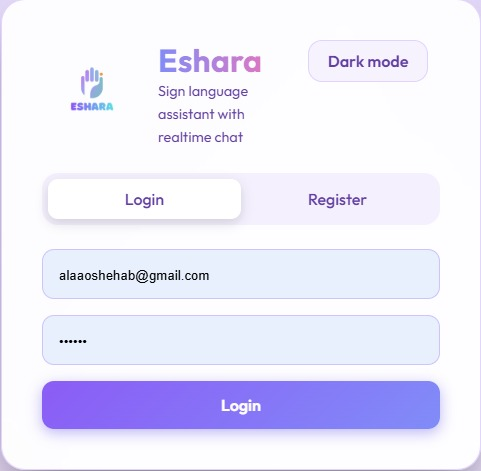
\includegraphics[width=0.54\textwidth]{images/fig_7-8_login_screen.png}
\caption{Eshara Landing Page: logo, tagline, Login/Register toggle, dark-mode switch, and credential form.}
\label{fig:ch7-login}
\end{figure}
\vspace{0.2cm}

\begin{figure}[H]
\centering
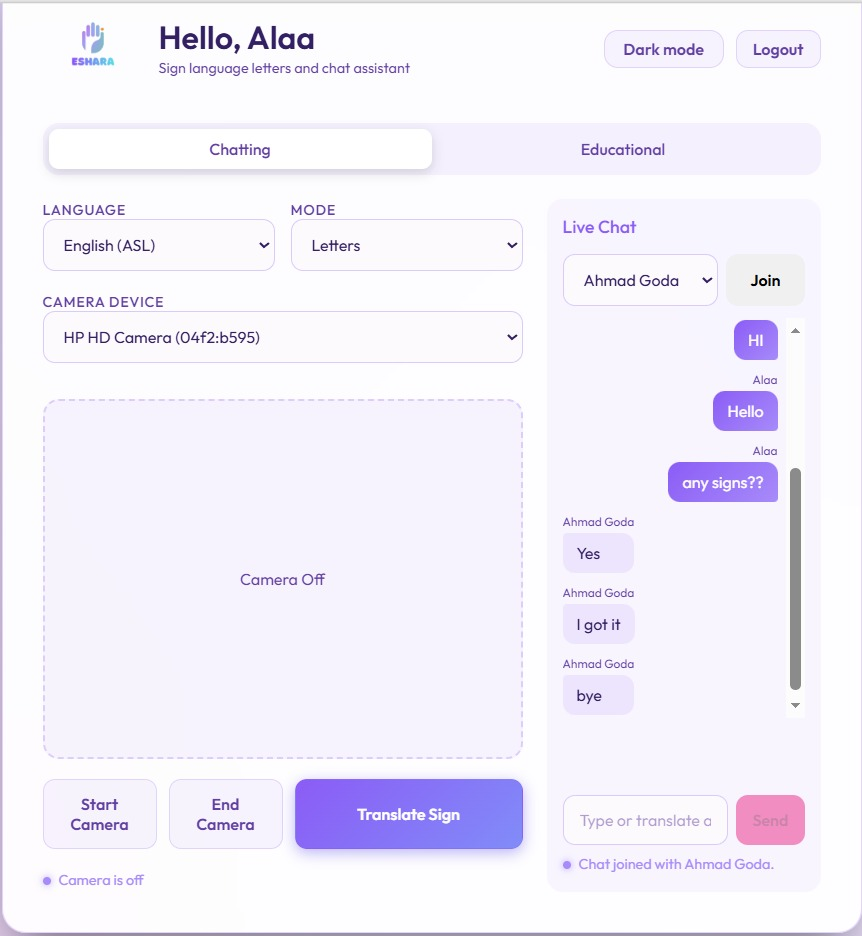
\includegraphics[width=0.54\textwidth]{images/fig_7-9_chat_translation_screen.png}
\caption{Eshara App Home Page (Chatting tab): language/mode/camera-device selectors, webcam capture panel with Start/End Camera and Translate Sign controls, and the Live Chat panel with an active Socket.IO room.}
\label{fig:ch7-apphome}
\end{figure}
\vspace{0.2cm}

\noindent\textbf{5.8\quad FEATURES, FUNCTIONALITY, AND UX DESIGN}\par
\addcontentsline{toc}{section}{\numberline{5.8}FEATURES, FUNCTIONALITY, AND UX DESIGN}
\vspace{0.1cm}

\noindent\textbf{Live chat and AI translation.} The flagship feature merges standard text messaging with AI-driven translation: the user selects a target language (ASL/ArSL) and scope (letters/words); the mirrored webcam feed lets the user see themselves naturally while signing; and, once a translation is produced, the predicted output is appended to the chat buffer and can be emitted to a live Socket.IO room, enabling cross-user communication carried out entirely in sign language.\par\vspace{0.1cm}

\noindent\textbf{Educational tools.} The Educational tab hosts three bilingual (ASL/ArSL) learning tools --- a categorised \textit{Sign Viewer} with integrated fingerspelling, a free-text \textit{Sentence Builder}, and a webcam \textit{Practice} mode --- built on motion-capture skeleton playback with server-side animation stitching; the module is documented in full in Section~5.14 (Part~B).\par\vspace{0.1cm}

\noindent\textbf{Responsive design and feedback.} CSS media queries and a flexible \texttt{display: grid} layout let the interface adapt fluidly from desktop monitors to small mobile viewports, stacking side-by-side panels (camera feed and chat window) vertically on constrained screens~\cite{wcag22}. Every interaction gives immediate visual feedback: translation requests trigger a temporary \textit{``Translating\ldots''} state, and socket connections display \textit{``Connected''} or \textit{``Error''} banners; modern micro-animations are used sparingly to keep the interface responsive without clutter.\par\vspace{0.3cm}

\noindent\textbf{5.9\quad SECURITY CONSIDERATIONS}\par
\addcontentsline{toc}{section}{\numberline{5.9}SECURITY CONSIDERATIONS}
\vspace{0.1cm}

\noindent\textbf{Authentication and cryptography.} User passwords are never stored in plaintext; they are hashed with \texttt{bcryptjs} using a high salt round before insertion into the database~\cite{bcrypt2024}. Sessions are managed statelessly via JWTs, so authentication tokens are cryptographically signed and tamper-evident~\cite{rfc7519}.\par\vspace{0.1cm}

\noindent\textbf{Encapsulated ML tier.} The FastAPI model service is explicitly hidden behind the Node.js application server; because the ML service ports are never exposed to the public internet, the attack surface is significantly reduced and every translation request must pass through the Node.js authentication middleware before reaching the inference engine.\par\vspace{0.1cm}

\noindent\textbf{CORS and input validation.} Cross-Origin Resource Sharing is strictly configured on the backend to prevent unauthorised domains from calling the APIs, and input payloads --- particularly login credentials and large base64 image strings --- are validated before processing to mitigate injection attacks and buffer-overload abuse. Transmitting landmark vectors rather than raw video for the letter and ArSL-word paths (Chapter~2, Chapter~7 Section~7.6) further reduces the amount of biometric image data that ever leaves the client for two of the four models; the ASL word path, which must transmit RGB frames for the I3D network, does not carry this benefit and is discussed as a residual privacy trade-off in Chapter~7.\par

\clearpage
\noindent\textbf{5.10\quad DEPLOYMENT}\par
\addcontentsline{toc}{section}{\numberline{5.10}DEPLOYMENT}
\vspace{0.2cm}

\noindent Graduation deployment is \textbf{web-only} across three independently hostable tiers: the React SPA is served as a static build over HTTPS; the Node.js + Express application server runs as a long-lived process with its SQLite database file on a persistent volume and the Socket.IO server attached to the same HTTP instance; and the FastAPI service runs in an isolated ML inference environment with the four model checkpoints loaded from disk. No app-store packaging, React Native wrapper, or on-device TensorFlow Lite/PyTorch Mobile export is part of the graduation deliverable.\par\vspace{0.2cm}

\begin{figure}[H]
\centering
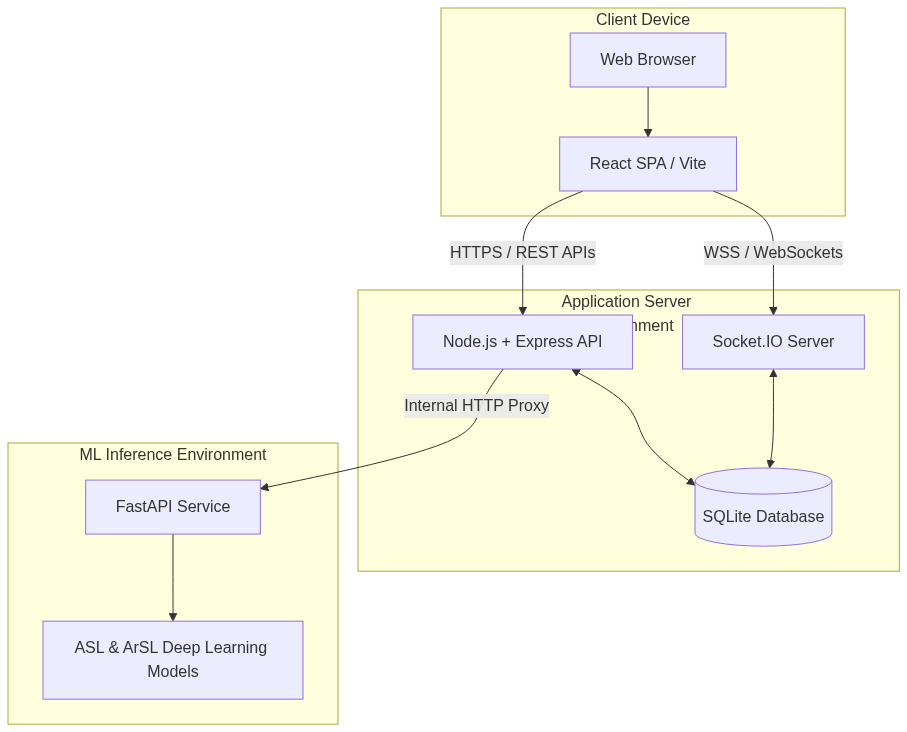
\includegraphics[width=1.10\textwidth]{images/fig_7-7_deployment_diagram.png}
\caption{Deployment diagram: client device (browser, React SPA) communicating over HTTPS/REST and WSS/WebSockets with the application server (Node.js + Express, Socket.IO, SQLite), which forwards inference requests over an internal HTTP proxy to the isolated ML inference environment (FastAPI service, ASL/ArSL deep-learning models).}
\label{fig:ch7-deployment}
\end{figure}
\vspace{0.3cm}

\noindent\textbf{5.11\quad ERROR HANDLING AND TESTING}\par
\addcontentsline{toc}{section}{\numberline{5.11}ERROR HANDLING AND TESTING}
\vspace{0.2cm}

\noindent\textbf{5.11.1\quad Graceful degradation:}\par
\addcontentsline{toc}{subsection}{\numberline{5.11.1}Graceful degradation:}
\vspace{0.2cm}

\noindent On the client, global Axios interceptors catch \texttt{401 Unauthorized} responses to purge invalid sessions and redirect the user, and browser APIs such as \texttt{navigator.mediaDevices} are wrapped in \texttt{try/catch} blocks so that a denied or missing webcam falls back to human-readable troubleshooting instructions rather than a silent failure. On the server, Express controllers wrap external calls in \texttt{try/catch}; if the FastAPI service is offline, the Node.js proxy catches the failed fetch and returns a structured \texttt{503 Service Unavailable} response instead of allowing the primary server process to crash.\par\vspace{0.2cm}

\noindent\textbf{5.11.2\quad Testing methodology:}\par
\addcontentsline{toc}{subsection}{\numberline{5.11.2}Testing methodology:}
\vspace{0.2cm}

\noindent The application underwent manual interface and integration testing covering real-time Socket.IO chat latency, responsive layout reflow on constrained mobile viewports, and cross-browser webcam access. Independently of the web integration, each backend ML model was evaluated against its own standardised dataset split before integration (Chapter~6); integration testing then confirmed that frontend JPEG base64 compression does not introduce artifacts that materially degrade active web inference paths during live webcam use.\par\vspace{0.3cm}

\noindent\textbf{5.12\quad REAL-TIME WEB PERFORMANCE}\par
\addcontentsline{toc}{section}{\numberline{5.12}REAL-TIME WEB PERFORMANCE}
\vspace{0.2cm}

\noindent Chapter~1 hypothesised end-to-end latency $\leq 200$\,ms from frame capture to displayed text on a standard laptop. As reported in the following table, \textbf{pilot measurements} on graduation development hardware (Windows 11 laptop, Chrome, 720p webcam, localhost stack) use 100 samples per row, timed with \texttt{performance.now()} in the browser and server wall-clock around \texttt{model.predict}; the full measurement protocol is documented in the project evaluation notes.\par\vspace{0.2cm}

\begin{table}[H]
\centering
\caption{Real-time web performance (pilot measurements, graduation dev hardware).}
\label{tab:ch7-latency}
\small
\begin{tabular}{|l|l|c|c|}
\hline
\multicolumn{1}{|c|}{\textbf{Component}} & \multicolumn{1}{|c|}{\textbf{How measured}} & \multicolumn{1}{|c|}{\textbf{p50}} & \multicolumn{1}{|c|}{\textbf{p95}}\\
\hline
MediaPipe (FastAPI, server-side) & 100 frames, server wall-clock around landmark extraction & 34 ms ($\sim$29 FPS) & 48 ms \\
\hline
Server inference (letter MLP) & FastAPI timing around predict & 4 ms & 7 ms \\
\hline
Server inference (ArSL word BiLSTM) & 48-frame batch (offline-validated path) & 24 ms & 38 ms \\
\hline
Server inference (ASL word I3D) & 32-frame RGB batch (CUDA) & 92 ms & 128 ms \\
\hline
HTTP \texttt{/predict} round-trip (letter) & Client POST $\rightarrow$ Node proxy $\rightarrow$ JSON response & 11 ms & 19 ms \\
\hline
\textbf{E2E letter} & Frame $\rightarrow$ UI label update & \textbf{51 ms} & 74 ms \\
\hline
\textbf{E2E ArSL word (offline-validated)} & FastAPI inference after 48-frame buffer & 41 ms & 68 ms \\
\hline
\textbf{E2E ASL word} & Inference after 32-frame buffer & 108 ms & 145 ms \\
\hline
\end{tabular}
\end{table}
\vspace{0.3cm}

\noindent Letter mode satisfies the $\leq 200$\,ms hypothesis (p50\,=\,51\,ms). Word modes incur an additional \textbf{buffer-fill} delay ($\sim$1.0--1.6\,s at 30\,FPS for 32--48 frames) before the first inference; per-commit server latency remains below 150\,ms. Server-side MediaPipe extraction dominates the letter-path compute budget before the MLP forward pass; letter MLP inference remains under 5\,ms on CPU as expected from Chapter~3 architecture size. ArSL word rows in Table~\ref{tab:ch7-latency} reflect the offline-validated FastAPI path documented in Section~5.5.3, not the current mock web response for \texttt{arabic + words}.\par\vspace{0.3cm}

\noindent\textbf{5.13\quad INFORMAL USABILITY PILOT}\par
\addcontentsline{toc}{section}{\numberline{5.13}INFORMAL USABILITY PILOT}
\vspace{0.2cm}

\noindent A formal deaf-community study with System Usability Scale (SUS) scoring was out of graduation scope (Chapter~6, Section~6.6). An \textbf{informal pilot} ($N{=}3$ student testers, 15-minute sessions each) exercised all four modes in the React UI. The following table records structured observations; a full SUS study with 10+ participants is recommended in Chapter~9~\cite{wcag22}.\par\vspace{0.2cm}

\begin{table}[H]
\centering
\caption{Informal usability pilot observations ($N{=}3$, React web UI).}
\label{tab:ch7-usability}
\small
\begin{tabular}{|l|c|l|}
\hline
\multicolumn{1}{|c|}{\textbf{Criterion}} & \multicolumn{1}{|c|}{\textbf{Rating}} & \multicolumn{1}{|c|}{\textbf{Notes}}\\
\hline
Camera setup ($<$1 min) & Good & Standard browser permission flow \\
\hline
Letter mode clarity & Good & Stabilisation reduces flicker; J/Z motion weak \\
\hline
ArSL word mode clarity & Good & 48-frame buffer requires full sign duration \\
\hline
ASL word mode clarity & Fair & Framing sensitivity; 32-frame window \\
\hline
RTL Arabic display & Good & Sentence builder readable \\
\hline
Mode switching (letter/word) & Fair & Manual toggle; no auto-detection \\
\hline
Overall assistive potential & Good & Suitable for practice, not certified interpretation \\
\hline
\end{tabular}
\end{table}
\vspace{0.2cm}

\clearpage
\begin{center}{\large \textbf{PART B --- EDUCATION MODULE}}\end{center}
\vspace{0.1cm}

\noindent\textbf{5.14\quad EDUCATION MODULE: BILINGUAL SIGN-LANGUAGE LEARNING}\par
\addcontentsline{toc}{section}{\numberline{5.14}EDUCATION MODULE: BILINGUAL SIGN-LANGUAGE LEARNING}
\vspace{0.2cm}

\noindent This section documents the Education tab at the same technical depth as Part~A's Translation \& Chat features. The module was rebuilt during the final development cycle around \textbf{motion-capture skeleton playback}: signs are no longer drawn as hand-authored stick-figure keyframes but replayed from pose recordings of real signers, and the module grew from two ASL practice panels into three bilingual learning tools. In both American Sign Language and Arabic Sign Language the tab offers a \textbf{Sign Viewer} (browse a categorised vocabulary and watch each sign, or fingerspell any typed word), a \textbf{Sentence Builder} (type a free-form sentence and watch it signed end-to-end), and a \textbf{Practice} mode (perform a prompted sign into the webcam and get instant feedback from the same recognition models that power the Chatting tab). Unlike the earlier canvas-only iteration, the Education tab is now a client--server feature: animation assembly runs in the FastAPI model-services tier, which stitches multiple sign clips into one smooth animation and streams it to the browser.\par\vspace{0.3cm}

\noindent\textbf{5.14.1\quad Overview and layout:}\par
\addcontentsline{toc}{subsection}{\numberline{5.14.1}Overview and layout:}
\vspace{0.2cm}

\noindent The Education tab is one of the two primary tabs on the App Home Page alongside Chatting (Section~5.7). A header sub-navigation carries a language toggle --- \textit{ASL~$\cdot$~English} / \textit{ArSL~$\cdot$~\arTxt{العربية}} --- and a tool switch between the Sign Viewer, the Sentence Builder, and Practice mode. Switching languages remounts the tool components with a React \texttt{key=\{lang\}}, so selection, playback, and camera state reset naturally without manual synchronisation logic. Each component receives its language-specific configuration (word list, categories, alphabet, text direction, placeholder copy) from a single \texttt{LANG\_CONFIG} lookup, so the English and Arabic experiences share one code path.\par\vspace{0.2cm}

\begin{figure}[H]
\centering
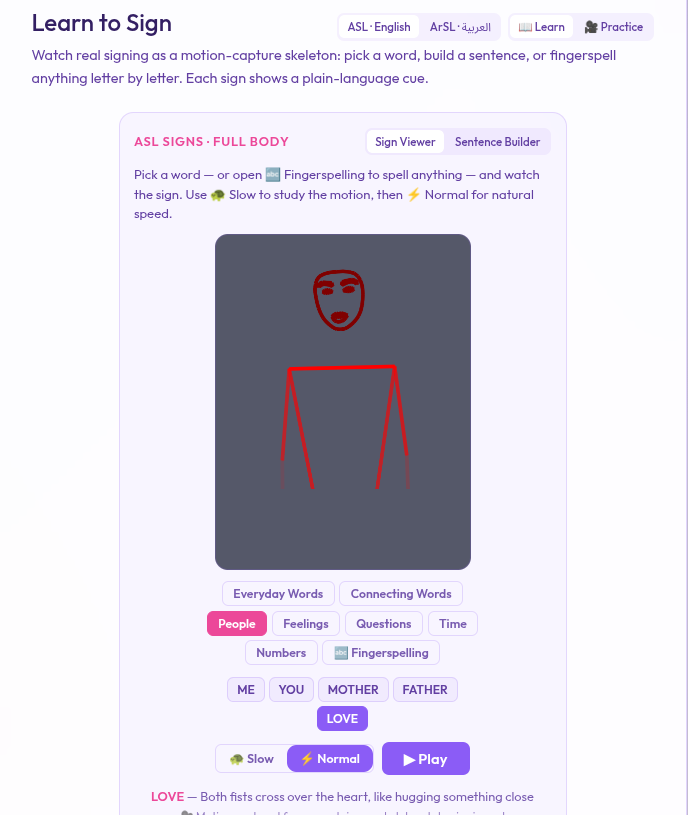
\includegraphics[width=0.62\textwidth]{images/fig_5-10_education.png}
\caption{Eshara Education tab (Sign Viewer, ASL): motion-capture skeleton playback with categorised vocabulary and playback-speed controls.}
\label{fig:ch5-edu-viewer}
\end{figure}
\vspace{0.2cm}

\noindent\textbf{5.14.2\quad Motivation: from hand-authored keyframes to motion capture:}\par
\addcontentsline{toc}{subsection}{\numberline{5.14.2}Motivation: from hand-authored keyframes to motion capture:}
\vspace{0.2cm}

\noindent An earlier iteration of this module rendered signs with a bespoke Canvas2D stick figure: every sign was a manually authored sequence of wrist keyframes and procedurally constructed handshapes, resolved through a two-joint inverse-kinematics solver. That engine was fast and dependency-free, but it could not scale in either quantity or quality. Each new sign required careful manual authoring and a geometric verification pass (hands visually merging, contact points floating off the head), the vocabulary plateaued at fifteen words, and even a correct keyframe animation reads as a symbolic illustration rather than a human performing the sign --- a material pedagogical weakness for a learning tool.\par\vspace{0.2cm}

\noindent The module was therefore rebuilt on \textbf{skeleton recordings of real signers}. Every sign is a \texttt{.pose} file --- the standard binary format of the \texttt{pose-format} library~\cite{poseformat} --- containing per-frame MediaPipe Holistic landmarks (body, face, and both hands) extracted from video of a human signer~\cite{zhang2020mediapipe}, replayed in the browser by the \texttt{<pose-viewer>} web component from the sign-language-processing project (the same renderer used by the open-source sign.mt translation platform~\cite{signmt2023}). This reversal of the earlier decision to avoid \texttt{<pose-viewer>} was deliberate and evidence-based: the lag that originally motivated the Canvas2D rewrite was caused not by the renderer itself but by playing many small clips back-to-back with client-side fetches between them. The rebuilt module fixes the root cause with server-side animation stitching (Section~5.14.4) --- one continuous animation per Play press --- while gaining human motion data, per-finger articulation, and a content pipeline that can grow the vocabulary without manual animation work. The legacy canvas stickman remains only as a fallback renderer for the few English words that have hand-authored keyframes but no \texttt{.pose} file.\par\vspace{0.3cm}

\noindent\textbf{5.14.3\quad Content pipeline: dictionary signs from sign.mt:}\par
\addcontentsline{toc}{subsection}{\numberline{5.14.3}Content pipeline: dictionary signs from sign.mt:}
\vspace{0.2cm}

\noindent Sign content is fetched offline from sign.mt's public dictionary API (\texttt{model-services/fetch\_signmt\_pose.py}), which translates a spoken-language word into a signed-language pose clip drawn from a curated dictionary: American Sign Language (\texttt{ase}) for English and Jordanian Sign Language (\texttt{jos}) for Arabic --- the only openly available Arabic-lookup sign dictionary~\cite{signmt2023}. The deployed vocabulary counts 44 English words plus the 26-letter manual alphabet, and 42 verified Arabic word signs plus the 28-letter Arabic alphabet; every clip is attributed on-page (\textit{``Motion captured from a real signer''}). Critically, the API silently returns a \textbf{fingerspelled} letter sequence, with HTTP~200, for any word its dictionary does not contain --- so a successful fetch does not prove the dictionary has the sign. The verification methodology built to defeat this failure mode is documented in Section~5.14.8.\par\vspace{0.2cm}

\noindent One rendering subtlety is worth recording. The \texttt{pose-viewer} custom element upgrades lazily, and a false JSX boolean attribute is removed from the DOM entirely --- so \texttt{autoplay=\{false\}} never reaches the component, whose internal default is \texttt{true}. Each component therefore sets \texttt{el.autoplay = false} imperatively in a mount effect, and drives playback through the component's \texttt{play()}/\texttt{pause()} methods and its \texttt{loadeddata\$}~/~\texttt{ended\$} events.\par\vspace{0.3cm}

\noindent\textbf{5.14.4\quad Server-side animation stitching (\texttt{pose\_concat.py}):}\par
\addcontentsline{toc}{subsection}{\numberline{5.14.4}Server-side animation stitching (\texttt{pose\_concat.py}):}
\vspace{0.2cm}

\noindent Playing letter or word clips back-to-back on the client produced the original module's characteristic lag: between every two clips the skeleton snapped from one pose to another, with a network fetch in between. All multi-sign playback was therefore moved server-side. The FastAPI tier stitches the requested signs into \textbf{one} \texttt{.pose} file using \texttt{spoken-to-signed} --- sign.mt's own concatenation package~\cite{spokentosigned} --- and streams the finished animation to the client:
\begin{enumerate}
\item Each clip is reduced (redundant landmarks dropped), normalised, and trimmed at its natural signing boundaries (a wrist-above-elbow heuristic finds where signing actually starts and ends).
\item Adjacent clips are cut at their best \textbf{connection point} --- the frame pair where the two skeletons are geometrically closest --- so one sign flows into the next.
\item A short zero-confidence gap (0.2\,s) is inserted at every boundary and filled by interpolation; the whole sequence is then smoothed with a Savitzky--Golay filter, wrist positions are corrected, and the result is size-normalised.
\end{enumerate}
\vspace{0.1cm}

\noindent Three language-parameterised endpoint families expose this pipeline:
\begin{itemize}
\item \texttt{/api/pose-seq} (\texttt{mode=words}) --- stitches a list of named signs with natural trimmed motion; used when the Sign Viewer plays a word.
\item \texttt{/api/pose-seq} (\texttt{mode=spell}) --- fingerspelling mode. Letter clips are inconsistent upstream (some are 3-frame stills, some full 25/30\,fps clips), and connection-point cutting can shrink a letter to a few unreadable frames --- so spell mode instead slices each letter to its central held handshape and freezes it for 0.35\,s, producing a uniform, readable spelling rhythm.
\item \texttt{/api/pose-text} --- free-text mode for the Sentence Builder (Section~5.14.6).
\end{itemize}
\vspace{0.1cm}

\noindent Every stitching endpoint has a \texttt{/meta} twin returning per-segment durations on the final timeline; because the animation itself is a single opaque file, synchronised UI feedback (highlighting the word chip or letter currently playing) is driven entirely by this metadata with plain client-side timers. Results are memoised server-side (\texttt{functools.lru\_cache}) so a repeated Play press is a cache hit, and \texttt{Content-Disposition} headers use RFC~5987 encoding because Arabic filenames cannot be represented in latin-1 HTTP headers. Sentence input is bounded (12 tokens, 80 stitched segments) so a pathological request cannot exhaust the service.\par\vspace{0.3cm}

\noindent\textbf{5.14.5\quad Sign Viewer:}\par
\addcontentsline{toc}{subsection}{\numberline{5.14.5}Sign Viewer:}
\vspace{0.2cm}

\noindent The Sign Viewer presents the language's vocabulary as category tabs (\textit{Everyday Words}, \textit{People}, \textit{Feelings}, \ldots; \arTxt{كلمات يومية}, \arTxt{الناس}, \arTxt{مشاعر وصفات}, \ldots) with one button per word. Selecting a word previews its first frame; Play streams the sign at \textit{Slow} (0.5$\times$) or \textit{Normal} (1$\times$, the default) speed, and each word is captioned with its meaning --- for Arabic, an English gloss, since the app's UI language is English. A final tab, \textit{Fingerspelling}, replaces the word grid with a letter reference grid (A--Z for ASL; the 28 Arabic base letters for ArSL) whose buttons play each letter's held handshape, plus a free spelling input: any typed word is filtered to spellable letters and played as one server-stitched spell-mode sequence, with the on-screen grid highlighting each letter in sync via the \texttt{/meta} timing data. If the configured default word is ever pruned from the vocabulary, the component falls back to the first available word rather than rendering an empty viewer.\par\vspace{0.2cm}

\begin{figure}[H]
\centering
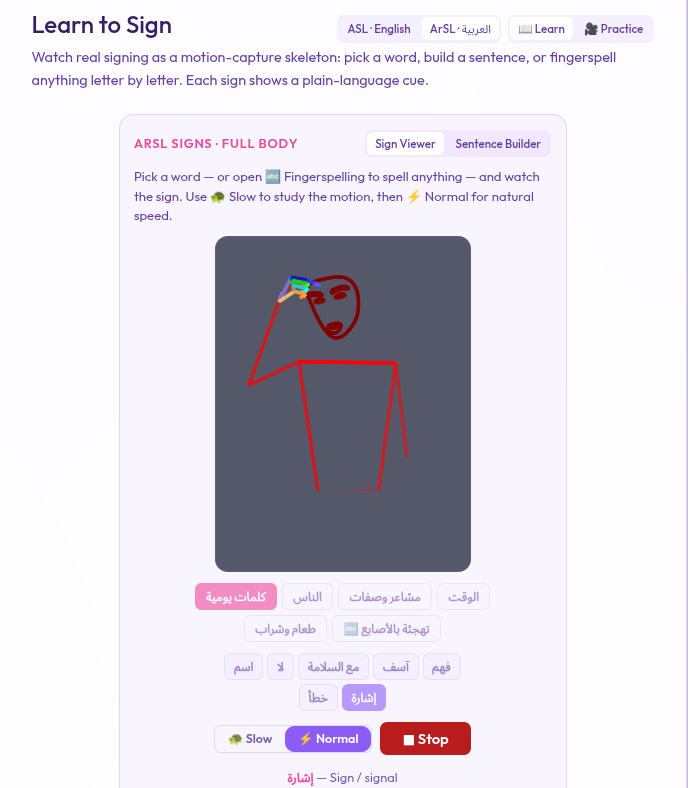
\includegraphics[width=0.62\textwidth]{images/fig_5-11_education.png}
\caption{Sign Viewer (ArSL): Jordanian Sign Language skeleton playback with right-to-left category and word controls.}
\label{fig:ch5-edu-arsl}
\end{figure}

\begin{figure}[H]
\centering
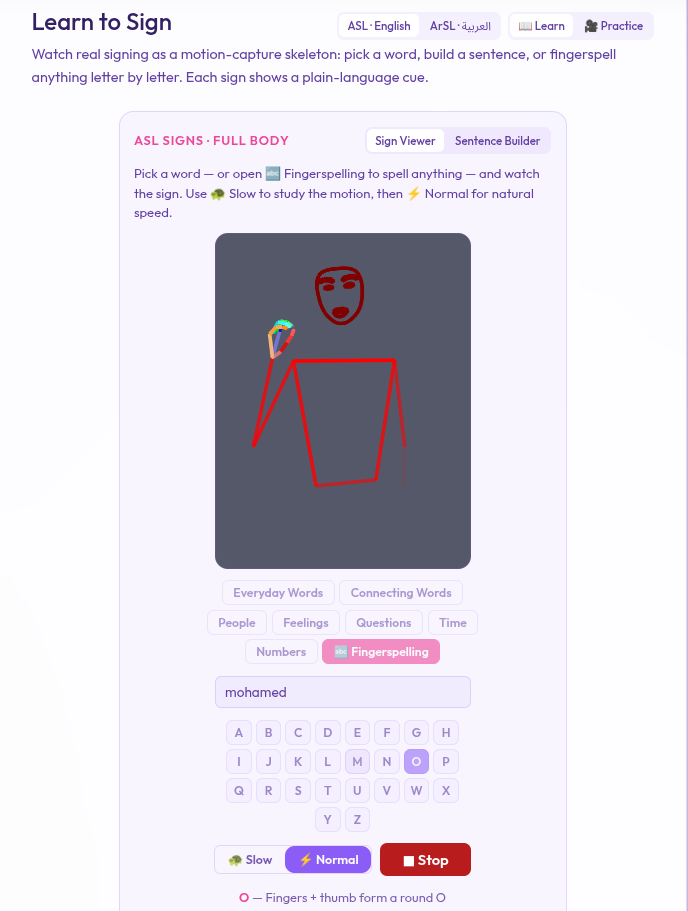
\includegraphics[width=0.62\textwidth]{images/fig_5-12_education.png}
\caption{Fingerspelling: a typed word plays as one server-stitched sequence while the current letter is highlighted from timing metadata.}
\label{fig:ch5-edu-spell}
\end{figure}
\vspace{0.2cm}

\noindent\textbf{5.14.6\quad Sentence Builder --- free-text signing:}\par
\addcontentsline{toc}{subsection}{\numberline{5.14.6}Sentence Builder --- free-text signing:}
\vspace{0.2cm}

\noindent The Sentence Builder follows sign.mt's interaction model: the user types any sentence; words found in the sign dictionary are signed, and unknown words are fingerspelled letter by letter~\cite{signmt2023}. The server's plan builder (\texttt{pose\_concat.build\_text\_sequence}) implements this as follows:
\begin{enumerate}
\item The text is tokenised (lowercased; Arabic diacritics stripped; digits 1--5 and Arabic-Indic \arTxt{١}--\arTxt{٥} mapped to their number words).
\item Tokens are matched greedily against the dictionary, longest phrase first (3-gram, then 2-gram, then single word) --- multi-word entries such as \textit{``thank you''} or \arTxt{مع السلامة} exist as \textbf{one} pose file and must not be split into unknown singles and spelled.
\item Lookups are orthography-tolerant (Section~5.14.7): both the query and the stored filenames are folded before comparison.
\item Any token still unmatched is decomposed into its letters and fingerspelled inline, using the same held-peak treatment as the Fingerspelling tab.
\item The full plan is stitched into one smooth animation and returned with per-token and per-letter timing metadata.
\end{enumerate}
\vspace{0.1cm}

\noindent The frontend mirrors the same greedy matching client-side to render a live \textbf{chip preview} as the user types: solid chips are words that will be signed from the dictionary; dashed chips carrying a fingerspelling marker will be spelled. This honesty matters --- a learner must never mistake a spelled word for the word's actual sign. During playback the chips and, for spelled tokens, the individual letters light up in sync with the animation.\par\vspace{0.2cm}

\begin{figure}[H]
\centering
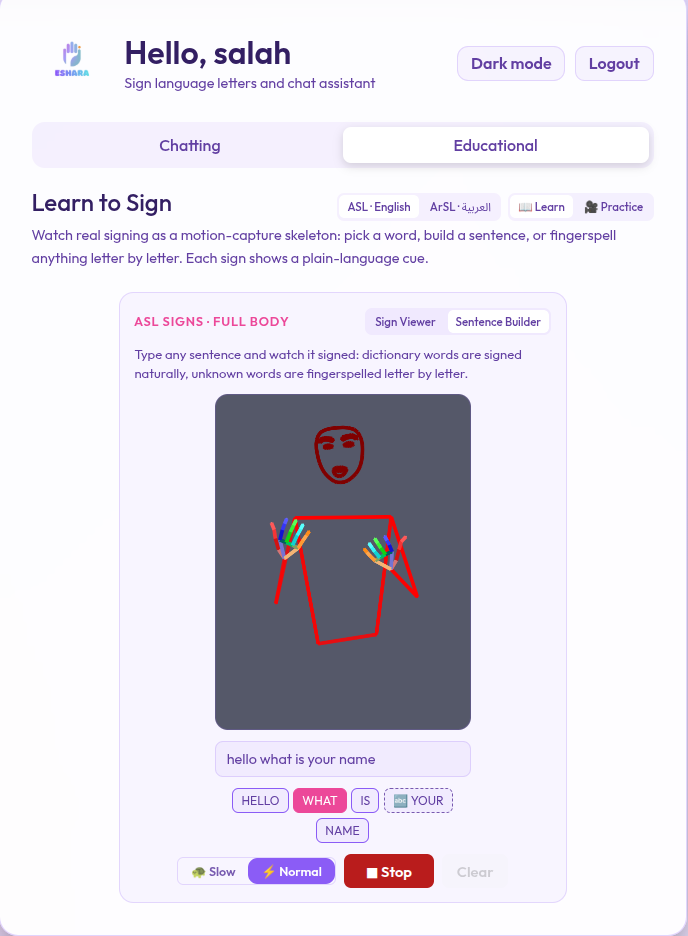
\includegraphics[width=0.62\textwidth]{images/fig_5-13_education.png}
\caption{Sentence Builder: dictionary words render as solid chips and are signed; unknown words render as dashed chips and are fingerspelled, with live highlighting driven by timing metadata.}
\label{fig:ch5-edu-sentence}
\end{figure}
\vspace{0.2cm}

\noindent\textbf{5.14.7\quad Arabic support (ArSL):}\par
\addcontentsline{toc}{subsection}{\numberline{5.14.7}Arabic support (ArSL):}
\vspace{0.2cm}

\noindent Every pose endpoint takes \texttt{lang=en|ar} and resolves content from a per-language directory. The tools are fully parameterised for Arabic: right-to-left text direction on inputs and labels, Arabic-Indic digit handling, and Arabic category labels. Two Arabic-specific engineering problems are worth recording:
\begin{itemize}
\item \textbf{Orthographic variance.} Arabic words are commonly typed without hamza/madda marks (\arTxt{ام} for \arTxt{أم}, \arTxt{اسف} for \arTxt{آسف}), yet the sign dictionary keys many entries under proper orthography --- and vice versa. A single folding table (\arTxt{أ}\,\arTxt{إ}\,\arTxt{آ}\,$\rightarrow$\,\arTxt{ا}; \arTxt{ى}\,\arTxt{ئ}\,$\rightarrow$\,\arTxt{ي}; \arTxt{ؤ}\,$\rightarrow$\,\arTxt{و}; \arTxt{ة}\,$\rightarrow$\,\arTxt{ه}; \arTxt{ء} dropped) is applied to \textbf{both} sides of every lookup: the server resolves queries through a folded-name index, and the client mirrors the same fold for chip previews and practice-answer matching. Files keep their proper spellings; users may type either form.
\item \textbf{Fingerspelling alphabet.} ArSL fingerspelling uses the 28 base letters; variant forms fold onto the letters that have clips (e.g.\ \arTxt{ة} spells as \arTxt{ه}), and diacritics are stripped before spelling.
\end{itemize}
\vspace{0.1cm}

\noindent Two linguistic caveats are documented for the record. First, the Arabic sign content is Jordanian Sign Language (\texttt{jos}) --- the only openly available Arabic sign dictionary --- while the ArSL recognition models were trained on KArSL (Saudi) data~\cite{sidig2021karsl}; regional sign variants differ, so the viewer and the recogniser are not guaranteed to agree on every word. Second, sentence signing follows the typed word order (a transliteration); it does not reorder into natural sign-language grammar. Both are acceptable for a learning aid but are stated honestly in the interface and in this thesis.\par\vspace{0.3cm}

\noindent\textbf{5.14.8\quad Content verification --- defeating the silent fallback:}\par
\addcontentsline{toc}{subsection}{\numberline{5.14.8}Content verification --- defeating the silent fallback:}
\vspace{0.2cm}

\noindent The hardest data-quality problem in the module was the dictionary API's silent fallback: for an out-of-vocabulary word it returns a fingerspelled letter sequence that is indistinguishable, at the protocol level, from a real sign. Publishing such a clip as a word sign would teach learners something actively wrong, and visual review alone proved unreliable --- a reviewer who does not know Jordanian Sign Language cannot always tell an unfamiliar sign from a spelled sequence. An automated classifier was therefore built:
\begin{enumerate}
\item For a candidate word, fetch the word itself \textbf{and} the doubled word (the word concatenated with itself). The doubled form is guaranteed to be out-of-vocabulary, so its returned animation is, by construction, the cloud's own spelling of the word, processed by the identical pipeline.
\item Reduce both animations to per-frame \textbf{handshape descriptors}: the 21 right-hand landmarks, wrist-relative and scale-normalised, so global position and size differences cancel.
\item Compare with start-anchored \textbf{dynamic time warping} (DTW), which absorbs the timing differences the stitching pipeline introduces. If the word's animation matches the spelling's prefix, it \textbf{is} the spelling fallback. Scores separate cleanly: spelled $<0.9$, real $\geq 2.9$.
\end{enumerate}
\vspace{0.1cm}

\noindent Every accepted clip was additionally reviewed frame-by-frame as a rendered filmstrip. A sweep of roughly 170 candidate Arabic words produced two further discoveries. First, the dictionary keys many entries under proper orthography only --- \arTxt{أم} is a real sign while \arTxt{ام} comes back spelled --- which directly motivated the fold-everywhere lookup of Section~5.14.7. Second, words containing \arTxt{ة} crash the API with HTTP~500 when out-of-vocabulary (its spelling lexicon lacks that letter), which turns the status code into a truth oracle for that word class. The final Arabic vocabulary --- verified word signs only --- is exactly the set that passed all checks; everything else fingerspells honestly with the dashed-chip treatment.\par\vspace{0.3cm}

\noindent\textbf{5.14.9\quad Practice mode --- learn by doing:}\par
\addcontentsline{toc}{subsection}{\numberline{5.14.9}Practice mode --- learn by doing:}
\vspace{0.2cm}

\noindent Practice mode closes the learning loop: after watching a sign, the user performs it. The panel reuses the exact camera-and-predict pipeline that powers the live Chatting tab --- extracted into a shared \texttt{useCamera} hook --- with its own camera instance so the two tabs never interfere:
\begin{itemize}
\item \textbf{Letter practice:} the panel prompts a random letter; the user poses it and a single webcam frame is sent to \texttt{POST /predict} (\texttt{mode=letters}). The models return exactly the comparison target --- an uppercase English letter or a real Arabic glyph --- so matching is a normalised string comparison.
\item \textbf{Word practice:} the panel prompts a word, runs a 3-2-1 countdown (cued performance needs reaction time), records a 3.2-second clip, and sends it to \texttt{POST /predict} (\texttt{mode=words}). Arabic matching folds orthography on both sides so the model's bare-spelled labels (\arTxt{انا}) match the vocabulary's proper spellings (\arTxt{أنا}).
\item \textbf{Honest target lists:} only words the deployed checkpoints can actually recognise are offered for checking --- the education words inside the WLASL-100 class list for ASL, and the fold-normalised intersection with the KArSL model's labels for ArSL. Everything else is watch-only rather than silently impossible.
\item \textbf{Constructive feedback:} when the model saw a sign but stayed below its confidence threshold, the UI reports its best guess (\textit{``it looked like X, just not clearly enough''}) instead of a generic failure, distinguishing \textit{``almost had it''} from \textit{``wrong sign entirely''}.
\end{itemize}
\vspace{0.1cm}

\begin{figure}[H]
\centering
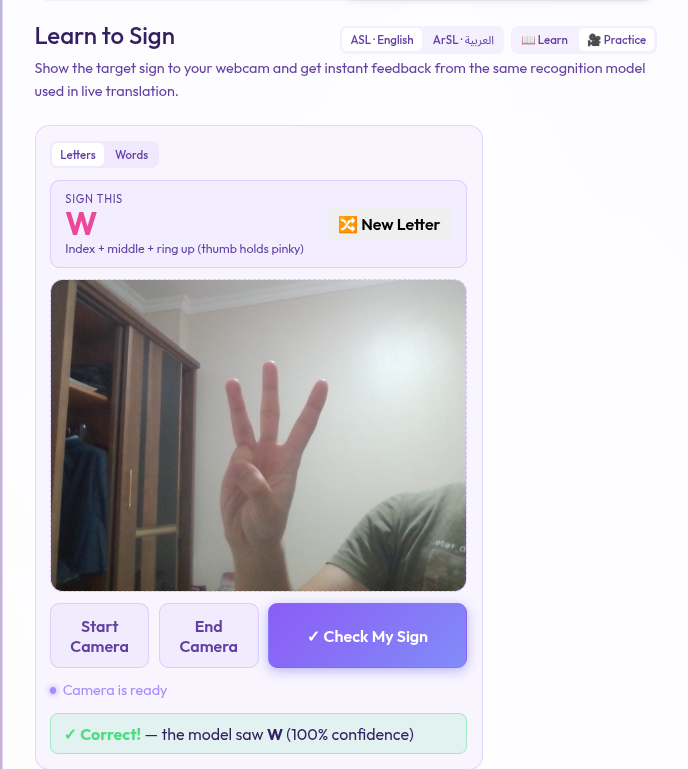
\includegraphics[width=0.62\textwidth]{images/fig_5-14_education.png}
\caption{Practice mode: the learner performs a prompted sign; the same recognition models that power live translation check the attempt and give constructive feedback.}
\label{fig:ch5-edu-practice}
\end{figure}
\vspace{0.2cm}

\noindent\textbf{5.14.10\quad Performance and verification engineering:}\par
\addcontentsline{toc}{subsection}{\numberline{5.14.10}Performance and verification engineering:}
\vspace{0.2cm}

\noindent Four decisions keep the rebuilt module responsive and correct; the following table contrasts the deployed pipeline with the superseded Canvas2D engine.
\begin{itemize}
\item \textbf{One stitched file per playback.} All multi-sign animation is assembled server-side and cached, so the client performs exactly one media fetch per Play press regardless of sentence length --- the root-cause fix for the original choppy, per-clip playback.
\item \textbf{A single persistent viewer element.} Each tool keeps one \texttt{<pose-viewer>} mounted across word and tab switches (hidden when the canvas fallback is active), so switching words never re-initialises the rendering component; idle previews load only the first frame.
\item \textbf{Guarded interaction states.} Word buttons, letter grids, and inputs are disabled during playback; playback promises resolve on the component's \texttt{ended\$} event, a cancellation poll, or a hard timeout, so the UI can never wedge in a playing state.
\item \textbf{End-to-end browser verification.} Every change to the module was verified in a scripted headless Chrome session (Playwright): log in as a QA user, drive the real UI --- switch language, play specific words, type sentences, assert chip classifications --- and require zero browser console errors. Sign-content changes were additionally verified by rendering filmstrip sheets of the actual pose data and reviewing them visually.
\end{itemize}
\vspace{0.1cm}

\begin{table}[H]
\centering
\caption{Education module: superseded Canvas2D engine versus the deployed motion-capture pipeline.}
\label{tab:ch5-edu-renderers}
\small
\begin{tabular}{|P{3.1cm}|P{5.2cm}|P{5.6cm}|}
\hline
\multicolumn{1}{|c|}{\textbf{Property}} & \multicolumn{1}{c|}{\textbf{Superseded (Canvas2D)}} & \multicolumn{1}{c|}{\textbf{Deployed (motion capture)}}\\
\hline
Rendering & Hand-authored keyframes + two-joint IK stick figure & \texttt{<pose-viewer>} skeleton playback of \texttt{.pose} recordings \\
\hline
Animation source & In-repo keyframes authored by the team (15 words, ASL only) & Dictionary recordings of real signers via sign.mt (44 EN + 42 AR words, both alphabets) \\
\hline
Multi-sign playback & Per-letter client sequencing & One server-stitched animation with timing metadata for UI highlights \\
\hline
Bilingual coverage & ASL only & Full ASL/ArSL parity incl.\ RTL and orthography-folded lookup \\
\hline
Correctness assurance & Manual geometric review of keyframes & DTW fallback detection + filmstrip review + scripted zero-console-error browser tests \\
\hline
\end{tabular}
\end{table}
\vspace{0.2cm}

\noindent\textbf{Part B summary.} The Education module pairs three tools --- a categorised Sign Viewer with integrated fingerspelling, a free-text Sentence Builder, and a webcam Practice mode --- across two sign languages behind one bilingual architecture. Signs are motion-capture skeletons of real signers, rendered by the \texttt{pose-viewer} web component and stitched server-side into single smooth animations whose timing metadata drives synchronised UI highlights. Arabic support required orthography-folded lookup on both client and server, right-to-left interface treatment, and a rigorous DTW-based verification methodology to reject the dictionary API's silent fingerspelling fallbacks --- ensuring that every word the module presents as a sign is genuinely that sign, and that everything else is honestly labelled as fingerspelling. Practice mode closes the loop by checking the learner's own signing against the same recognition models that power live translation, offering only targets those models can actually recognise.\par\vspace{0.3cm}

\clearpage
\noindent\textbf{Chapter summary.} Chapter~5 documented Eshara's realisation as a three-tier web product in two parts. \textbf{Part~A} covered a React/Vite client for capture, visualisation, and chat; a Node.js/Express application server providing JWT authentication, Prisma/SQLite persistence, and Socket.IO real-time messaging; and a FastAPI model-services tier that dispatches base64 frames to the active ASL/ArSL letter and ASL-word inference paths, including the PyTorch Inception I3D integration for ASL words with per-session frame buffering. Security is layered through bcrypt password hashing, stateless JWT sessions, an encapsulated ML tier, and CORS/input validation; error handling degrades gracefully on both client and server. Pilot measurements confirm letter-mode end-to-end latency meets the $\leq 200$\,ms target from Chapter~1 (Table~\ref{tab:ch7-latency}), and an informal three-tester usability pass (Table~\ref{tab:ch7-usability}) rates the system suitable for practice and assistive use, not certified interpretation. \textbf{Part~B} documented the Education Module: bilingual Sign Viewer, Sentence Builder, and Practice tools built on motion-capture skeleton playback (\texttt{pose-viewer}), server-side animation stitching with timing metadata, orthography-folded Arabic lookup, and a DTW-based content-verification methodology that rejects fingerspelling fallbacks. Chapter~8 concludes the thesis; Chapter~9 outlines continuous recognition, vocabulary expansion, and formal user studies as future work.\par
